\documentclass[24pt,serif,aspectratio=169]{beamer}

% Set the margins to be something normal.
% \usepackage[margin=1in]{geometry}

% Fun lists!
\usepackage{enumitem}
\usepackage{textcomp}
\setitemize{label=\textrightarrow, itemsep=0pt}

% Math symbols.
\usepackage{amsmath,amssymb,amsfonts,tikz,mathtools,pgfplots,nicefrac,enumitem}
\pgfplotsset{compat=newest}
\usetikzlibrary{shapes,arrows,positioning,calc}  
\usetikzlibrary{overlay-beamer-styles}

% No indents.
\setlength\parindent{0pt}
\setlength\parskip{1em}

\newcommand{\inverse}[1]{#1^{-1}}

% Symbols.
\newcommand{\R}{\mathbb{R}}
\newcommand{\N}{\mathbb{N}}
\newcommand{\Z}{\mathbb{Z}}
\newcommand{\Q}{\mathbb{Q}}
\renewcommand{\H}{\mathbb{H}}
\newcommand{\C}{\mathbb{C}}
\renewcommand{\P}{\mathbb{P}}

% Uncovering underbraces.
\newcommand<>{\uncoverubrace}[2]{%
  \onslide#3 \underbrace{ \onslide<1->%
  #1%
  \onslide#3 }_{#2} \onslide<1->%
}
\newcommand<>{\uncoverobrace}[2]{%
  \onslide#3 \overbrace{ \onslide<1->%
  #1%
  \onslide#3 }^{#2} \onslide<1->%
}


% Nice fonts :)
%\usepackage{tgschola}
\usefonttheme[onlymath]{serif}

\begin{document}
	\begin{frame}[c] \centering \Huge
		sequences let us do calculus!
	\end{frame}
	
	\begin{frame}[c]\centering \Large
		a \textit{sequence} is an \textit{indexed set} of \textit{objects}.
	\end{frame}
	
	\begin{frame}[c]\centering \Large
		$$ \{a_n\}_{n=1}^N = \{a_1, a_2, a_3, \dots, a_N\} $$
	\end{frame}
	
	\begin{frame}[c]\centering \Large
		we can make sequences \textit{in any space we want},\\ not just the real numbers $\R$.
	\end{frame}
	
	\begin{frame}[c]\centering \Large
		$$ \{a_n\}_{n=1}^\infty = \{a_1, a_2, a_3, \dots\} $$
	\end{frame}
	
	\begin{frame}[c] \centering \Large
		$$ \left\{\frac 1n\right\}_1^\infty = \left\{1, \frac 12, \frac 13, \frac 14, \dots \right\} $$
	\end{frame}
	
	\begin{frame}[c]
		\begin{figure}\centering
			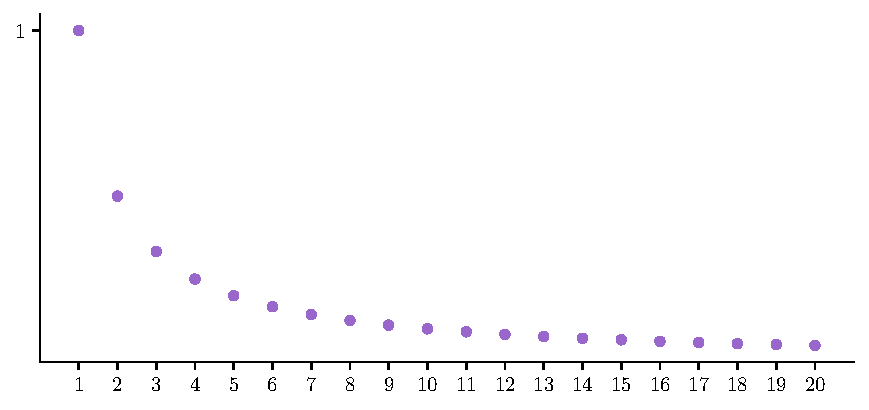
\includegraphics[width=\linewidth]{figures/1n.pdf}	
		\end{figure}
	\end{frame}
	
	\begin{frame}[c]\centering \Large
		a sequence \textit{has a limit at} $L$ if the entries $a_n$ \\ get \textit{arbitrarily close to} $L$ as $n \to \infty$.
	\end{frame}
	
	\begin{frame}[c] \Large
		$$\lim_{n \to \infty} a_n = L$$	when:
		\begin{enumerate}[label=$\xhookrightarrow{}$]
			\onslide<2->{\item for every positive number $\epsilon$...}
			\onslide<3->{\item we can choose a big index $N$, where...}
			\onslide<4->{\item for every index $m$ bigger than $N$...}
			\onslide<5->{\item the distance from $a_m$ to $L$ is less than $\epsilon$.}
		\end{enumerate}
	\end{frame}
	
	\begin{frame}[c] \Large
		mathematically...
		
		$$\lim_{n \to \infty} a_n = L$$ $$ \iff $$ $$ \uncoverubrace<2->{\forall \epsilon > 0}{\mathclap{\text{\footnotesize for every positive number $\epsilon$}}}, \uncoverobrace<3->{\exists N \in \N}{\mathclap{\text{\footnotesize we can choose a big index $N$}}} \text{ s.t. } \uncoverubrace<4->{\forall m > N}{\mathclap{\text{\footnotesize where, for every $m$ bigger than $N$}}}, \uncoverobrace<5->{|a_m - L| < \epsilon}{\mathclap{\text{\footnotesize the distance from $a_m$ to $L$ is less than $\epsilon$.}}}$$
	\end{frame}
	
	\begin{frame}[c] \Large \centering
		$$ L = 0, \epsilon = 1/10 $$
		\onslide<2->{if we choose $N = 10$, then for $m > 10$,}
		\onslide<3->{$$ \frac{1}{m} = a_m \onslide<4->{<} a_N = \frac{1}{10}$$}
	\end{frame}
	
	\begin{frame}[c] \Large \centering
		\begin{align*}
			|a_N - L| &= \left\lvert \frac{1}{10} - 0 \right\rvert \\
			&= \frac{1}{10} \\
			&= \epsilon
		\end{align*}
	\end{frame}
	
	\begin{frame}[c] \Large \centering
		but...
			\begin{align*}
				|a_m - L| &= \left\lvert\frac 1m - 0 \right\rvert \\
				\onslide<2->{&< \left\lvert \frac{1}{10} - 0 \right\rvert \\}
				\onslide<3->{&= \frac{1}{10} \\}
				\onslide<4->{&= \epsilon}
			\end{align*}
	\end{frame}
	
	\begin{frame}[c]\Huge
		$$ |a_m - 0| < \epsilon $$	
	\end{frame}
	
	\begin{frame}[c]
		\begin{figure}
			\centering
			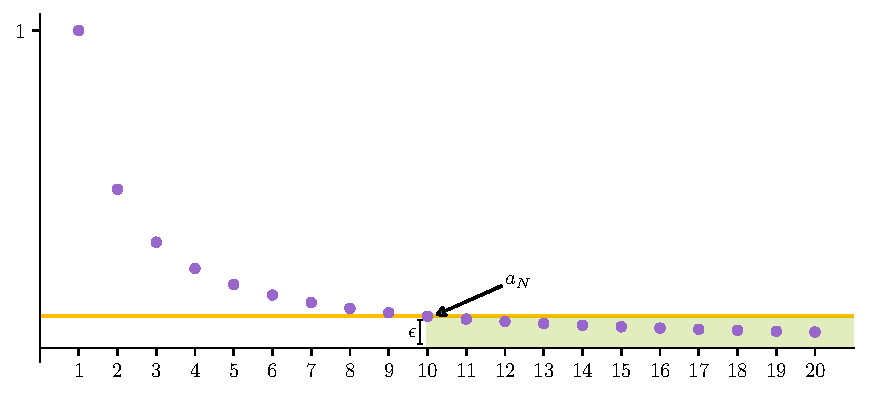
\includegraphics[width=\linewidth]{figures/1n-epsilon.pdf}	
		\end{figure}
	\end{frame}

	
	\begin{frame}[c]\Large \centering 
		if we can do this for \textit{every} $\epsilon > 0$... \\[2em] \onslide<2->{\Huge then our sequence converges to $0$.}
	\end{frame}
	
	\begin{frame}[c] \Large \centering
		big picture: \\[2em] our sequence has a limit at $L$ if the \\ elements \textit{eventually get really close to $L$.}	
	\end{frame}
	
	\begin{frame}[c] \Large \centering
		an important type of sequence is called a \textit{\LARGE Cauchy} sequence.	
	\end{frame}
	
	\begin{frame}[c] \Large \centering
		in a Cauchy sequence, the elements \\ get arbitrarily close to \textit{each other.}
	\end{frame}
	
	\begin{frame}[c] \Large
		$$\{a_n\}_{n=1}^\infty \text{ is Cauchy when:}$$
		\begin{enumerate}[label=$\xhookrightarrow{}$]
			\onslide<2->{\item for every positive number $\epsilon$...}
			\onslide<3->{\item we can choose a big index $N$, where...}
			\onslide<4->{\item for every index $p$ bigger than $N$ and every index $q$ bigger than $N$...}
			\onslide<5->{\item the distance from $a_p$ to $a_q$ is less than $\epsilon$.}
		\end{enumerate}
	\end{frame}
	
	\begin{frame}[c] \Large
		mathematically...
		$$\{a_n\}_{n=1}^\infty \text{ is Cauchy}$$ $$ \iff $$ $$ \uncoverubrace<2->{\forall \epsilon > 0}{\mathclap{\text{\footnotesize for every positive number $\epsilon$}}}, \uncoverobrace<3->{\exists N \in \N}{\mathclap{\text{\footnotesize we can choose a big index $N$}}} \text{ s.t. } \uncoverubrace<4->{\forall p, q > N†}{\mathclap{\text{\footnotesize where, for every $p$ and $q$ bigger than $N$}}}, \uncoverobrace<5->{|a_p-a_q| < \epsilon}{\mathclap{\text{\footnotesize the distance from $a_p$ to $a_q$ is less than $\epsilon$.}}}$$
	\end{frame}
	
	\begin{frame}[c] \LARGE
		$$ \left\{\sin\left(\frac{\pi \cdot n}{2}\right) \cdot e^{\frac{1/10}{n}} \right\}_{n=0}^\infty $$
	\end{frame}
	
	\begin{frame}[c]\centering
		\begin{figure}
			\centering
			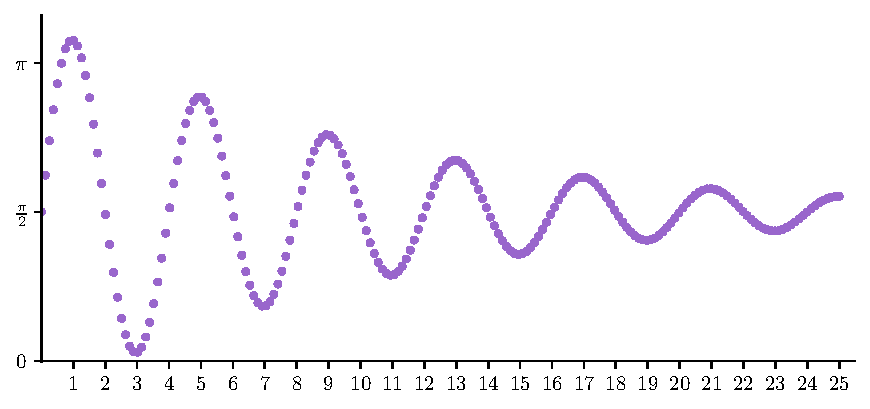
\includegraphics[width=\linewidth]{figures/sequence-cauchy-converges.pdf}	
		\end{figure}
	\end{frame}

	
	\begin{frame}[c]\centering \Large
		$$ N = 2, \epsilon = \frac \pi 2 $$
		$$ \implies |a_p - a_q| < \frac \pi 2 $$
		(when $p$ and $q$ are bigger than $2$)
	\end{frame}
	
	\begin{frame}[c]
		let $p = 5$ and $q = 7$:
		
		\begin{align*}	
			|a_p - a_q| \onslide<2->{&= \left\lvert \sin\left(\frac{\pi \cdot 5}{2}\right) \cdot e^{\frac{1/10}{5}} - \sin\left(\frac{\pi \cdot 7}{2}\right) \cdot e^{\frac{1/10}{7}}	\right\rvert \\}
			\onslide<3->{&\approx |2.177 - 1.074| \\}
			\onslide<4->{&= 1.103 \\}
			\onslide<5->{&< \frac \pi 2 \hspace{1em} (\approx 1.5708)\\}
			\onslide<6->{&= \epsilon}
		\end{align*}
	\end{frame}
	
	\begin{frame}[c]\centering
		\begin{figure}
			\centering
			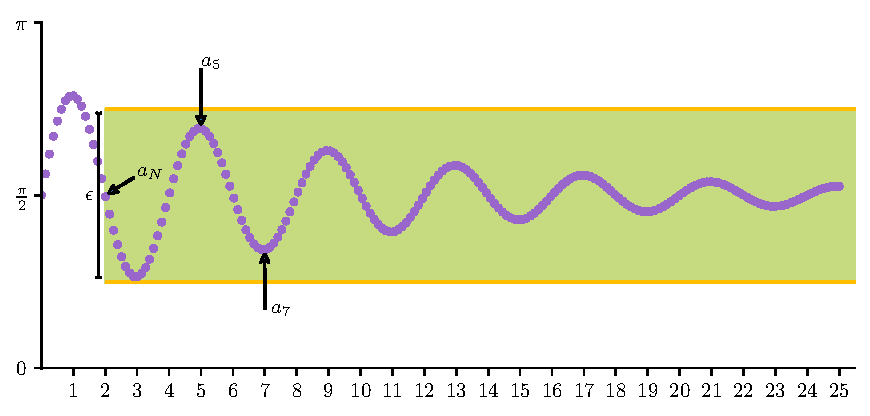
\includegraphics[width=\linewidth]{figures/sequence-cauchy-converges-annotated.pdf}
		\end{figure}
	\end{frame}
	
	\begin{frame}[c]\centering
		\begin{figure}
			\centering
			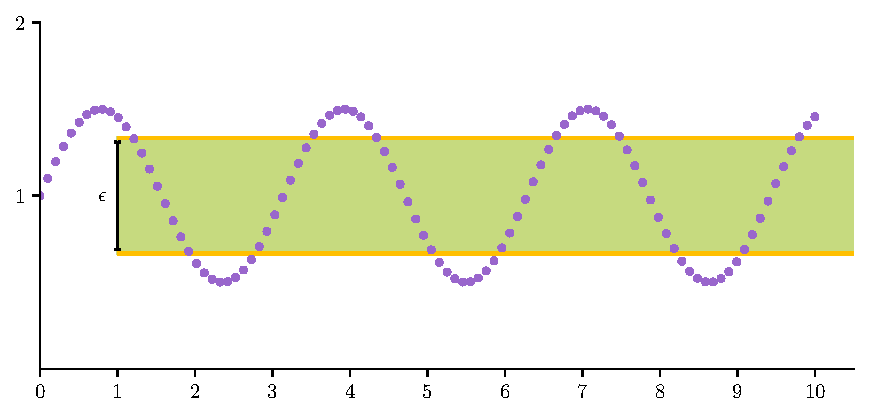
\includegraphics[width=\linewidth]{figures/sequence-cauchy-nothing.pdf}
		\end{figure}
	\end{frame}
	
	\begin{frame}[c]\centering \Large
		think about the sequence $$\{a_n\} = \{3, 3.1, 3.14, 3.141, 3.1415, 3.14159, \dots\}$$ \onslide<2->{$$ \lim_{n \to \infty} a_n = \pi$$}
	\end{frame}
	
	\begin{frame}[c]\Large \centering
		think about the function $f(x) = x^2$\onslide<2->{...\\ \textit{but force the domain of $f$ to be the rational numbers $\Q$.}}
	\end{frame}
	
	\begin{frame}[c]\Large \centering
		the \textit{intermediate value theorem} says that $$ \text{ on } [a,b] \text{, $f(x)$ takes on any value between $f(a)$ and $f(b)$ in } [a,b]. $$
	\end{frame}
	
	\begin{frame}[c]\Large \centering
		if $a=1$ and $b=2$, then $f(a) = 1$ and $f(b) = 4$... \onslide<2->{$$ f(a) < \pi < f(b) $$}
	\end{frame}
	
	\begin{frame}[c]\Huge \centering
		... but if we take $$\{f(\sqrt{a_n})\} = \{f(\sqrt{3}), f(\sqrt{3.14}), f(\sqrt{3.1415}), \dots\}$$
	\end{frame}
	
	\begin{frame}[c]\Huge \centering
		$$\lim_{n \to \infty} f(\sqrt{a_n}) = f(\sqrt \pi) = \pi $$ $$1 < \pi < 4$$ \onslide<2->{... but is $\pi$ a rational number?}
	\end{frame}
	
	\begin{frame}[c]\Huge \centering
		the intermediate value theorem \textit{fails.}
	\end{frame}
	
	\begin{frame}[c]\huge \centering
		the real numbers $\R$ are \textit{complete}: \\[2em]
		\onslide<2->{every Cauchy sequence converges to a real number.}
	\end{frame}

\end{document}
